\section{Validación experimental del sistema}
\label{sec:validacion-experimental}

Esta sección evalúa el sistema de automatización MLOps mediante cuatro experimentos centrados en su comportamiento operativo: eficiencia de los recursos, gestión de la saturación, correspondencia entre ejecución virtual y hardware real, y reducción del tiempo total mediante paralelización. Las configuraciones completas de las variantes utilizadas se recogen en el Anexo~\ref{anexo:parametros-experimentos} (Anexo C).

La ejecución correcta de las fases software F01--F06 y de las fases F07--F08 sobre ESP32 no se trata como dos pruebas aisladas. Ambas comprobaciones están incorporadas en los experimentos posteriores: los experimentos 1, 2 y 4 ejercitan las fases software, mientras que el experimento 3 compara las fases hardware en entornos físicos y virtualizados. De este modo se evita repetir evidencias y la validación se concentra en resultados cuantificables.

La evaluación se estructura según los siguientes ejes:

\begin{itemize}
    \item \textbf{Eficiencia de recursos:} comparar el tiempo de una fase ligera y otra intensiva sobre ejecución local, GitHub Actions y los perfiles Kubernetes de 8 y 24 GiB.
    \item \textbf{Saturación y colas:} observar el comportamiento del sistema cuando el número de variantes simultáneas supera el máximo de runners disponible.
    \item \textbf{Correspondencia entre entorno virtual y real:} contrastar la duración y el resultado de F07 y F08 sobre ESP32 físico y sobre su alternativa virtualizada.
    \item \textbf{Valor de la paralelización:} medir la reducción del \textit{lead time} al ejecutar un mismo árbol de variantes de forma secuencial y concurrente.
\end{itemize}

\subsection{Especificaciones de los entornos de ejecución}
\label{subsec:entornos-ejecucion}

Para interpretar los resultados experimentales se resumen los entornos utilizados durante la validación. La comparación no pretende medir únicamente la potencia bruta de cada máquina, sino relacionar cada tipo de runner con el componente del pipeline que ejecuta, su capacidad de paralelización y sus restricciones de acceso a hardware.

\subsubsection{Entorno local}
\label{subsubsec:entorno-local-validacion}

El entorno local se utiliza como referencia para comparar la ejecución directa del pipeline frente a la ejecución automatizada mediante runners externos. Este entorno permite comprobar que los resultados obtenidos en integración continua son coherentes con los obtenidos al lanzar las fases manualmente desde una máquina de desarrollo.

En la validación, este entorno se usa principalmente como punto de comparación para ejecuciones secuenciales y para contrastar tiempos frente a GitHub Actions y Kubernetes. Al no depender de colas ni de aprovisionamiento dinámico, permite aislar el tiempo propio de ejecución de cada fase.

\begin{table}[htbp]
    \centering
    \caption{Especificaciones del entorno local utilizado como referencia.}
    \label{tab:entorno-local-validacion}
    \begin{tabular}{p{0.28\textwidth}p{0.62\textwidth}}
        \hline
        \textbf{Elemento} & \textbf{Especificación} \\
        \hline
        Equipo & MSI PS42 Modern 8RA \\
        CPU & Intel Core i7-8565U, 8 hilos, hasta 4.60 GHz \\
        GPU & NVIDIA GeForce MX250 e Intel UHD Graphics 620 \\
        Memoria RAM & 15.46 GiB \\
        Sistema operativo & Omarchy 4.0.0.alpha \\
        Kernel & Linux 7.0.9-arch2-1 \\
        Uso experimental & Referencia manual y ejecución secuencial \\
        \hline
    \end{tabular}
\end{table}

\subsubsection{Runners hospedados por GitHub Actions}
\label{subsubsec:entorno-github-actions-validacion}

Los runners hospedados por GitHub Actions se emplean como entorno base para ejecutar fases software cuando no se requiere infraestructura propia ni acceso a hardware físico. En esta validación se utiliza la etiqueta \texttt{ubuntu-latest}, que selecciona una imagen Ubuntu mantenida por GitHub y ejecutada sobre una máquina virtual efímera.

Este entorno resulta útil como referencia externa porque elimina dependencias de la infraestructura local. Sin embargo, al tratarse de un runner efímero y gestionado por GitHub, la comparación se realiza sobre el perfil de recursos documentado y no sobre un modelo físico concreto de procesador.

\begin{table}[htbp]
    \centering
    \caption{Especificaciones consideradas para runners hospedados por GitHub Actions.}
    \label{tab:entorno-github-actions-validacion}
    \begin{tabular}{p{0.28\textwidth}p{0.62\textwidth}}
        \hline
        \textbf{Elemento} & \textbf{Especificación} \\
        \hline
        Tipo de runner & GitHub-hosted standard runner \\
        Etiqueta utilizada & \texttt{ubuntu-latest} \\
        Arquitectura & x64 \\
        CPU asignada & 4 vCPU \\
        Memoria RAM & 16 GB \\
        Almacenamiento SSD & 14 GB \\
        Modelo de ejecución & Máquina virtual efímera por job \\
        Uso experimental & Fases software F01--F06 \\
        Fuente & Perfil documentado por GitHub \cite{github_hosted_runners} \\
        \hline
    \end{tabular}
\end{table}

\subsubsection{Runners desplegados sobre Kubernetes}
\label{subsubsec:entorno-kubernetes-validacion}

Los runners sobre Kubernetes se utilizan para ejecutar cargas software sobre infraestructura propia con capacidad de escalado. Este entorno permite lanzar varias variantes en paralelo y ajustar el perfil de recursos según el coste esperado de cada componente del pipeline.

Durante la validación se consideran dos perfiles principales. El perfil \texttt{K8s-8gb} está orientado a componentes ligeros o a lotes con alto paralelismo, mientras que el perfil \texttt{K8s-24gb} se reserva para fases con mayor demanda de CPU o memoria. La comparación entre ambos no se limita al tiempo individual de ejecución, sino que también tiene en cuenta el número máximo de runners simultáneos.

\begin{table}[htbp]
    \centering
    \caption{Perfiles de runners Kubernetes utilizados durante la validación.}
    \label{tab:entorno-kubernetes-validacion}
    \begin{tabular}{p{0.18\textwidth}p{0.18\textwidth}p{0.18\textwidth}p{0.18\textwidth}p{0.18\textwidth}}
        \hline
        \textbf{Perfil} & \textbf{CPU solicitada} & \textbf{CPU límite} & \textbf{Memoria} & \textbf{Máx. runners} \\
        \hline
        \texttt{K8s-8gb} & 2 CPU & 4 CPU & 8 GiB & 5 \\
        \texttt{K8s-24gb} & 4 CPU & 8 CPU & 24 GiB & 3 \\
        \hline
    \end{tabular}
\end{table}

El clúster Kubernetes utilizado está formado por siete nodos Linux con arquitectura \texttt{amd64}. Todos los nodos ejecutan Debian GNU/Linux 12 (\textit{bookworm}), utilizan \texttt{containerd} como runtime de contenedores y ejecutan la versión \texttt{v1.36.0} de kubelet. La Tabla~\ref{tab:nodos-kubernetes-validacion} resume sus características principales.

\begin{table}[htbp]
    \centering
    \caption{Nodos del clúster Kubernetes utilizados durante la validación.}
    \label{tab:nodos-kubernetes-validacion}
    \begin{tabular}{p{0.13\textwidth}p{0.31\textwidth}p{0.09\textwidth}p{0.14\textwidth}p{0.13\textwidth}p{0.13\textwidth}}
        \hline
        \textbf{Nodo} & \textbf{Procesador} & \textbf{CPU} & \textbf{Memoria} & \textbf{Kernel} & \textbf{Runtime} \\
        \hline
        trasgo02 & Intel Xeon E5-2630 v2 @ 2.60GHz & 24 & 32863764 Ki & 6.1.0-45-amd64 & containerd 2.2.3 \\
        trasgo03 & Intel Xeon E5-2630 v2 @ 2.60GHz & 24 & 32863764 Ki & 6.1.0-45-amd64 & containerd 2.2.3 \\
        trasgo04 & Intel Xeon E5-2630 v2 @ 2.60GHz & 24 & 32863764 Ki & 6.1.0-45-amd64 & containerd 2.2.3 \\
        trasgo05 & Intel Xeon E5-2630 v2 @ 2.60GHz & 24 & 32863760 Ki & 6.1.0-42-amd64 & containerd 2.2.3 \\
        trasgo06 & Intel Xeon E5-2630 v2 @ 2.60GHz & 24 & 32863760 Ki & 6.1.0-42-amd64 & containerd 2.2.3 \\
        trasgo07 & Intel Xeon E5-2630 v2 @ 2.60GHz & 24 & 32863752 Ki & 6.1.0-42-amd64 & containerd 2.2.3 \\
        trasgo08 & Intel Xeon E5-2630 v2 @ 2.60GHz & 24 & 32863760 Ki & 6.1.0-42-amd64 & containerd 2.2.3 \\
        \hline
    \end{tabular}
\end{table}

Esta separación en perfiles permite estudiar el compromiso entre recursos por job y capacidad de paralelización, especialmente en experimentos con múltiples variantes concurrentes. Aunque todos los nodos presentan una configuración de CPU, memoria y sistema operativo muy similar, existen pequeñas diferencias en la versión del kernel, por lo que las comparaciones se interpretan a nivel de perfil de runner y no como una comparativa nodo a nodo.

\subsubsection{Runners autoalojados con ESP32}
\label{subsubsec:entorno-esp32-validacion}

Los runners con ESP32 se utilizan en las fases que requieren validación \textit{Hardware-in-the-Loop}. Estos runners están desplegados sobre un servidor Proxmox y se ejecutan dentro de contenedores LXC, cada uno con acceso al dispositivo ESP32 correspondiente mediante puerto serie.

Este entorno permite validar el comportamiento real de las fases F07 y F08, incluyendo la interacción con el microcontrolador y la obtención de métricas bajo condiciones próximas al despliegue final. A diferencia de GitHub Actions o Kubernetes, la disponibilidad del runner queda condicionada por el acceso físico al dispositivo.

\begin{table}[htbp]
    \centering
    \caption{Especificaciones de los runners autoalojados con ESP32.}
    \label{tab:entorno-esp32-validacion}
    \begin{tabular}{p{0.28\textwidth}p{0.62\textwidth}}
        \hline
        \textbf{Elemento} & \textbf{Especificación} \\
        \hline
        Servidor base & NucBox K10 sobre Proxmox VE 8.4.17 \\
        CPU del servidor & Intel Core i9-13900H de 13ª generación \\
        Memoria del servidor & 31.12 GiB RAM \\
        Contenedor runner & LXC con Debian 12 \\
        Recursos por contenedor & 2 CPU y 7 GiB RAM \\
        Acceso hardware & Puerto serie hacia ESP32 real \\
        Uso experimental & Fases F07--F08 \\
        \hline
    \end{tabular}
\end{table}

\subsection{Diseño de la validación y métricas}
\label{subsec:metodologia-validacion}

El diseño utiliza lotes controlados de variantes. Dentro de cada comparación se mantienen los parámetros funcionales y se modifica únicamente el factor estudiado: el runner, la capacidad disponible o el modo de ejecución. Para cada variante se registran:

\begin{itemize}
    \item el experimento, la fase, el identificador de variante y el runner asignado;
    \item la variante padre, utilizada para conservar las dependencias del pipeline;
    \item los instantes de creación, inicio y finalización;
    \item el tiempo de cola, el tiempo efectivo de ejecución y el tiempo total;
    \item el estado final de la ejecución.
\end{itemize}

La Tabla~\ref{tab:diseno-experimentos-validacion} resume las cuatro pruebas. La definición reproducible de cada lote, con sus parámetros, runners y relaciones padre-hija, se presenta en el Anexo~\ref{anexo:parametros-experimentos}. Los lotes base incluidos en ese anexo aportan las variantes previas necesarias, pero no se contabilizan como experimentos adicionales.

\begin{table}[htbp]
    \centering
    \caption{Diseño de los experimentos de validación.}
    \label{tab:diseno-experimentos-validacion}
    \begin{tabular}{p{0.10\textwidth}p{0.25\textwidth}p{0.36\textwidth}p{0.19\textwidth}}
        \hline
        \textbf{Exp.} & \textbf{Propósito} & \textbf{Comparación} & \textbf{Métricas} \\
        \hline
        1 & Eficiencia de recursos & F03 y F05 en Local, GitHub Actions, K8s-8gb y K8s-24gb & Tiempo de ejecución y capacidad paralela \\
        2 & Saturación & Ocho variantes F03 sobre K8s-8gb con cinco runners máximos & Cola, ejecución y tiempo total \\
        3 & Virtual frente a real & F07 y F08 en entornos ESP32 físicos y virtualizados & Tiempo de ejecución y estado final \\
        4 & Paralelización & Mismo árbol F01--F04 en modo secuencial y paralelo & \textit{Lead time}, aceleración y camino crítico \\
        \hline
    \end{tabular}
\end{table}

La corrección funcional actúa como condición previa en los cuatro experimentos: una variante solo se incorpora al análisis cuantitativo cuando finaliza con el estado esperado y conserva su relación con la variante padre. Por ello, la ejecución de las fases y la trazabilidad no se presentan como bloques independientes, sino como requisitos transversales de validez de las mediciones.

\subsection{Experimento 1: eficiencia de recursos}
\label{subsec:comparativa-entornos}

La comparativa de entornos estudia cómo varía el tiempo de ejecución cuando F03 y F05 se lanzan con los mismos parámetros sobre el entorno local, GitHub Actions y los perfiles Kubernetes de 8 y 24 GiB. Los runners con ESP32 no forman parte de este experimento, ya que se analizan específicamente en el Experimento 3.

La métrica utilizada es el tiempo efectivo de ejecución, registrado entre el inicio y la finalización de cada job mediante el campo \texttt{execution\_seconds}. Se excluye el tiempo previo de espera en cola para aislar, en la medida de lo posible, el rendimiento del entorno una vez asignado el runner. La gestión de la cola y su contribución al tiempo total se estudian de forma específica en el Experimento 2.

\subsubsection{Experimento 1.1: runners sobre GitHub Actions}
\label{subsubsec:exp11-runners-github-actions}

El primer bloque de esta comparativa analiza el comportamiento de los componentes software del pipeline cuando se ejecutan sobre runners gestionados desde GitHub Actions. El objetivo es disponer de una referencia reproducible y externa a la infraestructura propia, utilizando un entorno efímero creado para cada job.

En este experimento se consideran componentes representativos con distinta carga computacional. Por un lado, una fase ligera como \texttt{f03\_windows}, donde el coste principal está asociado al procesamiento de ventanas. Por otro lado, una fase más pesada como \texttt{f05\_modeling}, donde el entrenamiento de modelos incrementa el consumo de CPU, memoria y tiempo de ejecución.

\begin{table}[htbp]
    \centering
    \caption{Plantilla de resultados del Experimento 1.1 sobre runners de GitHub Actions.}
    \label{tab:exp11-github-actions}
    \begin{tabular}{llllll}
        \hline
        \textbf{Componente} & \textbf{Fase} & \textbf{Variante} & \textbf{Runner} & \textbf{Tiempo ejecución} & \textbf{Estado} \\
        \hline
        Ventanas & \texttt{f03\_windows} & [variante] & GitHub Actions & [s] & [estado] \\
        Modelado & \texttt{f05\_modeling} & [variante] & GitHub Actions & [s] & [estado] \\
        \hline
    \end{tabular}
\end{table}

\begin{figure}[htbp]
    \centering
    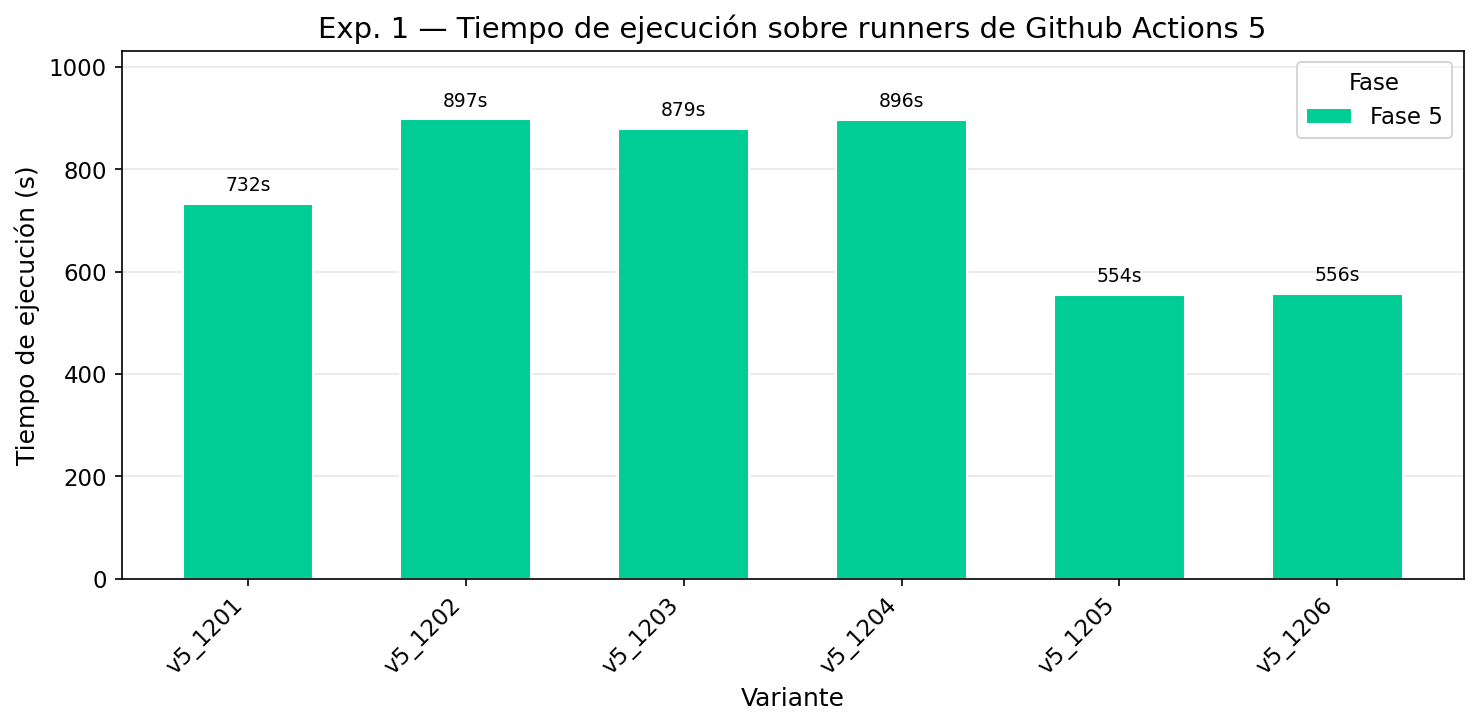
\includegraphics[width=0.95\textwidth]{figures/validacion/exp11_github_actions_componentes.png}
    \caption{Tiempos de ejecución por componente sobre runners de GitHub Actions en el Experimento 1.1.}
    \label{fig:exp11-github-actions}
\end{figure}

Esta prueba permite comprobar si GitHub Actions ofrece un comportamiento suficientemente estable para las fases software del pipeline y sirve como línea base frente a la infraestructura propia. Los resultados finales deberán indicar si la variabilidad observada es aceptable y qué fases son adecuadas para este tipo de runner.

\subsubsection{Experimento 1.2: runners del clúster Kubernetes con perfil K8s-8gb}
\label{subsubsec:exp12-runners-k8s-8gb}

El segundo bloque analiza la ejecución de componentes del pipeline sobre runners dinámicos del clúster Kubernetes con perfil \texttt{K8s-8gb}. Este perfil está orientado a ejecuciones ligeras o moderadas y permite un mayor grado de paralelización, ya que el número máximo de pods simultáneos es superior al del perfil de mayor memoria.

La prueba se plantea para comprobar si el perfil de 8 GiB es suficiente para componentes como \texttt{f03\_windows} y para estudiar su comportamiento cuando se utiliza también en fases más costosas. Además del tiempo efectivo de ejecución, se observa el estado final para detectar posibles limitaciones de recursos. La espera en cola no se incorpora a esta comparación.

\begin{table}[htbp]
    \centering
    \caption{Plantilla de resultados del Experimento 1.2 sobre runners K8s-8gb.}
    \label{tab:exp12-k8s-8gb}
    \begin{tabular}{llllll}
        \hline
        \textbf{Componente} & \textbf{Fase} & \textbf{Variante} & \textbf{Runner} & \textbf{Tiempo ejecución} & \textbf{Estado} \\
        \hline
        Ventanas & \texttt{f03\_windows} & [variante] & K8s-8gb & [s] & [estado] \\
        Modelado & \texttt{f05\_modeling} & [variante] & K8s-8gb & [s] & [estado] \\
        \hline
    \end{tabular}
\end{table}

\begin{figure}[htbp]
    \centering
    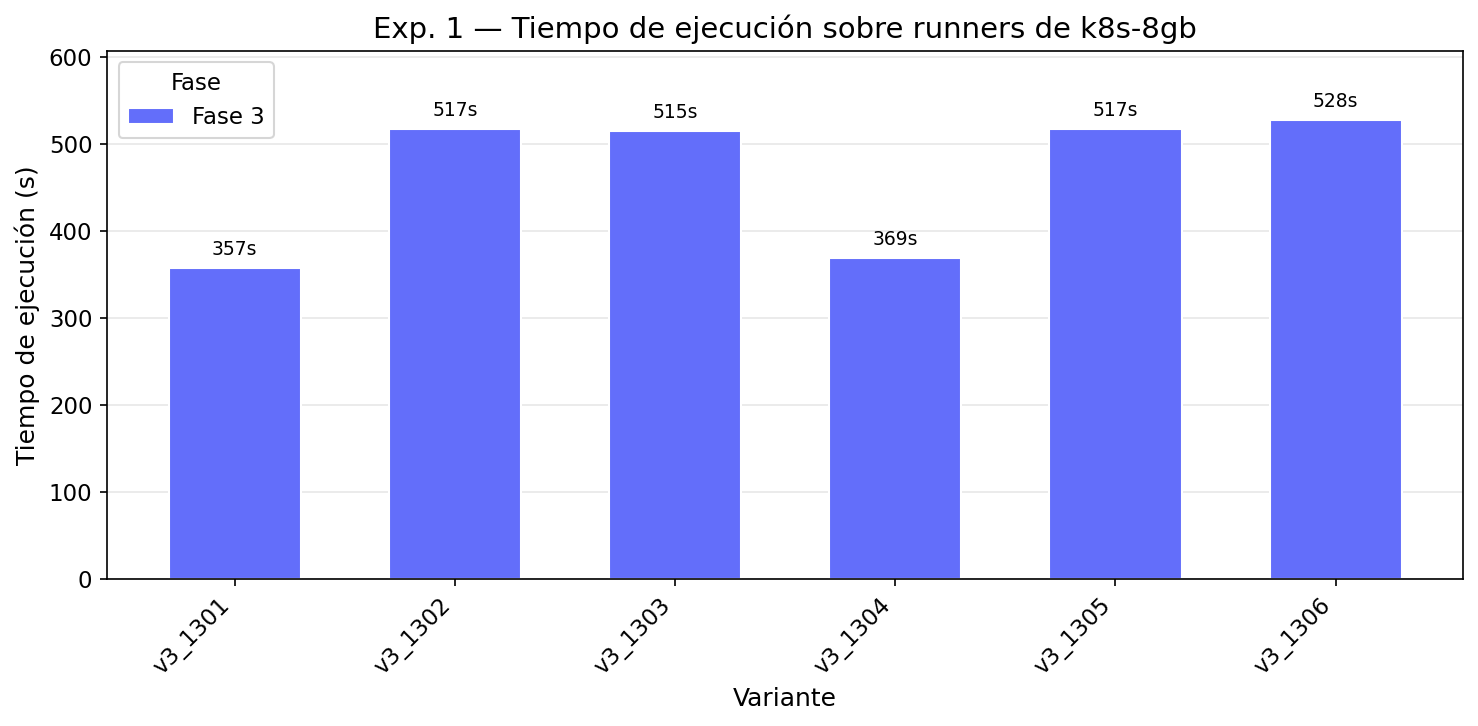
\includegraphics[width=0.95\textwidth]{figures/validacion/exp12_k8s_8gb_componentes.png}
    \caption{Tiempos de ejecución por componente sobre runners Kubernetes K8s-8gb en el Experimento 1.2.}
    \label{fig:exp12-k8s-8gb}
\end{figure}

El resultado esperado de este bloque es determinar qué componentes pueden ejecutarse de forma eficiente en el perfil ligero del clúster. Si el tiempo individual aumenta pero el paralelismo disponible permite ejecutar más variantes simultáneas, el análisis debe completarse con una métrica de \textit{throughput} efectivo.

\subsubsection{Experimento 1.3: repetición de componentes sobre K8s-8gb}
\label{subsubsec:exp13-runners-k8s-8gb-repeticion}

El tercer bloque mantiene el foco en el perfil \texttt{K8s-8gb}, pero lo utiliza como prueba de repetibilidad entre variantes del mismo componente. La intención es comprobar si varias ejecuciones equivalentes presentan tiempos similares o si aparecen diferencias relevantes debidas al arranque de pods, la distribución entre nodos del clúster o la carga concurrente del sistema.

Este experimento es útil para separar dos efectos distintos. Por una parte, permite medir la duración normal de un componente cuando se ejecuta sobre un runner Kubernetes ligero. Por otra, permite detectar si el entorno introduce variabilidad operativa suficiente como para afectar a la comparación entre variantes de modelo o de parámetros.

\begin{table}[htbp]
    \centering
    \caption{Plantilla de resultados del Experimento 1.3 de repetibilidad sobre K8s-8gb.}
    \label{tab:exp13-k8s-8gb-repeticion}
    \begin{tabular}{llllll}
        \hline
        \textbf{Componente} & \textbf{Fase} & \textbf{Variante} & \textbf{Runner} & \textbf{Tiempo ejecución} & \textbf{Observación} \\
        \hline
        Ventanas & \texttt{f03\_windows} & [variante] & K8s-8gb & [s] & [observación] \\
        Ventanas & \texttt{f03\_windows} & [variante] & K8s-8gb & [s] & [observación] \\
        Modelado & \texttt{f05\_modeling} & [variante] & K8s-8gb & [s] & [observación] \\
        \hline
    \end{tabular}
\end{table}

\begin{figure}[htbp]
    \centering
    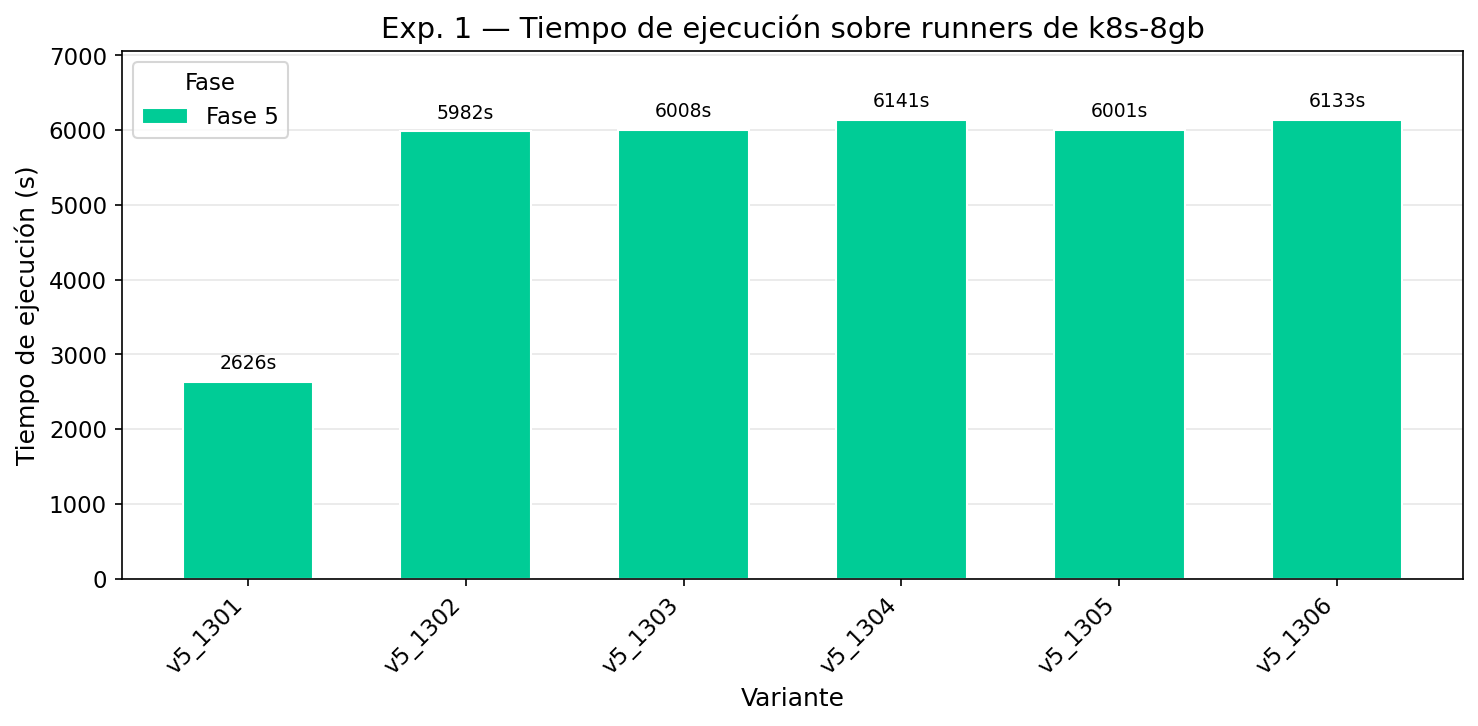
\includegraphics[width=0.95\textwidth]{figures/validacion/exp13_k8s_8gb_repetibilidad.png}
    \caption{Repetibilidad de tiempos de ejecución por componente sobre runners K8s-8gb en el Experimento 1.3.}
    \label{fig:exp13-k8s-8gb-repeticion}
\end{figure}

La interpretación de este experimento debe centrarse en la dispersión entre ejecuciones. Una dispersión baja indica que el runner es adecuado para comparar variantes experimentales. Una dispersión alta obliga a distinguir entre mejoras reales del pipeline y variabilidad introducida por la infraestructura.

\subsubsection{Experimento 1.4: runners del clúster Kubernetes con perfil K8s-24gb}
\label{subsubsec:exp14-runners-k8s-24gb}

El cuarto bloque evalúa el perfil \texttt{K8s-24gb}, orientado a componentes con mayor demanda de memoria o CPU. A diferencia del perfil \texttt{K8s-8gb}, este entorno dispone de más recursos por runner, pero permite un número menor de pods simultáneos. Por tanto, la comparación no debe limitarse al tiempo de una ejecución aislada, sino que debe considerar también la capacidad total del sistema para procesar lotes de variantes.

Este experimento es especialmente relevante para fases pesadas como \texttt{f05\_modeling}. Si el incremento de recursos reduce de forma significativa el tiempo de entrenamiento o evita fallos por memoria, el perfil de 24 GiB puede estar justificado. Si la mejora individual es pequeña, el perfil de 8 GiB puede ser preferible por su mayor paralelismo.

\begin{table}[htbp]
    \centering
    \caption{Plantilla de resultados del Experimento 1.4 sobre runners K8s-24gb.}
    \label{tab:exp14-k8s-24gb}
    \begin{tabular}{llllll}
        \hline
        \textbf{Componente} & \textbf{Fase} & \textbf{Variante} & \textbf{Runner} & \textbf{Tiempo ejecución} & \textbf{Estado} \\
        \hline
        Ventanas & \texttt{f03\_windows} & [variante] & K8s-24gb & [s] & [estado] \\
        Modelado & \texttt{f05\_modeling} & [variante] & K8s-24gb & [s] & [estado] \\
        \hline
    \end{tabular}
\end{table}

\begin{figure}[htbp]
    \centering
    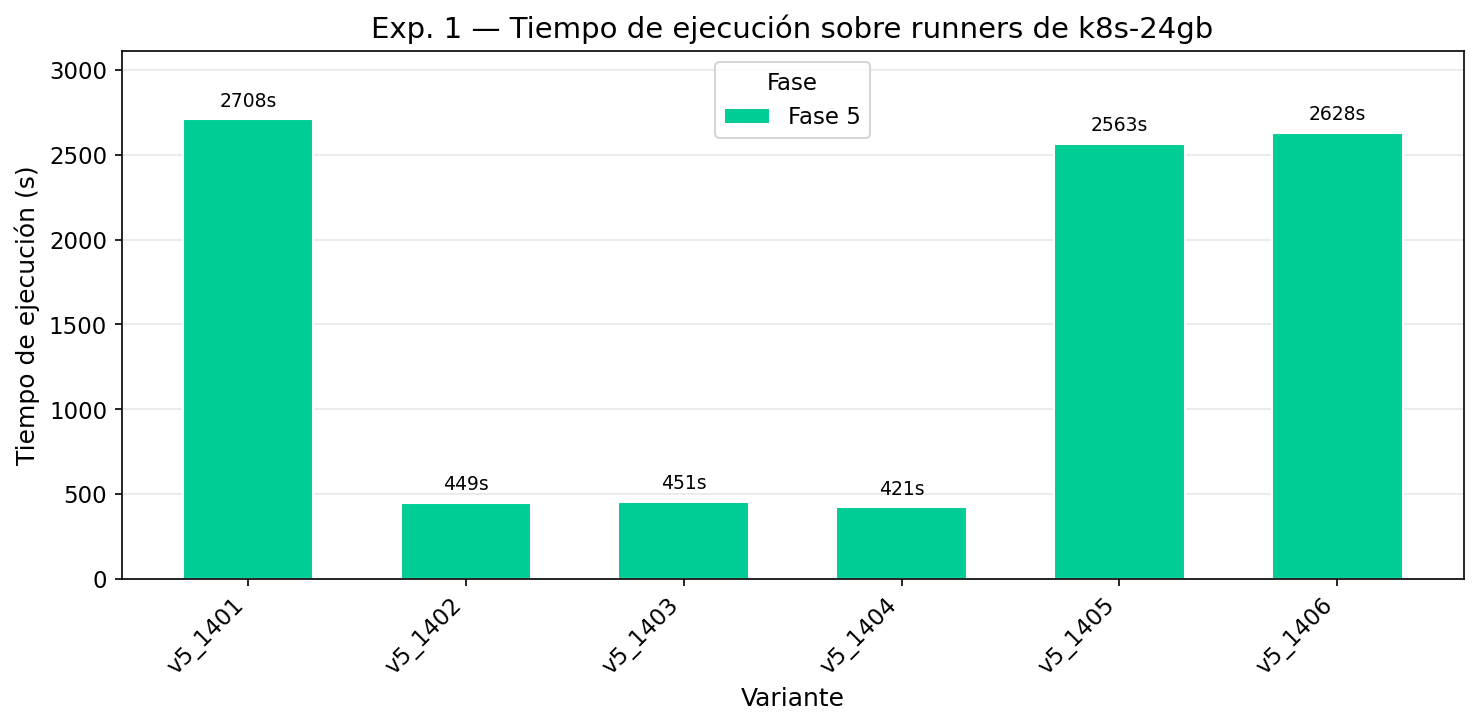
\includegraphics[width=0.95\textwidth]{figures/validacion/exp14_k8s_24gb_componentes.png}
    \caption{Tiempos de ejecución por componente sobre runners Kubernetes K8s-24gb en el Experimento 1.4.}
    \label{fig:exp14-k8s-24gb}
\end{figure}

La conclusión de este bloque debe comparar el perfil \texttt{K8s-24gb} con el perfil \texttt{K8s-8gb}, teniendo en cuenta tanto el tiempo de ejecución por componente como el paralelismo máximo disponible. Esta comparación permite justificar qué runner conviene asignar a cada componente del pipeline en función de su coste computacional.

\begin{figure}[htbp]
    \centering
    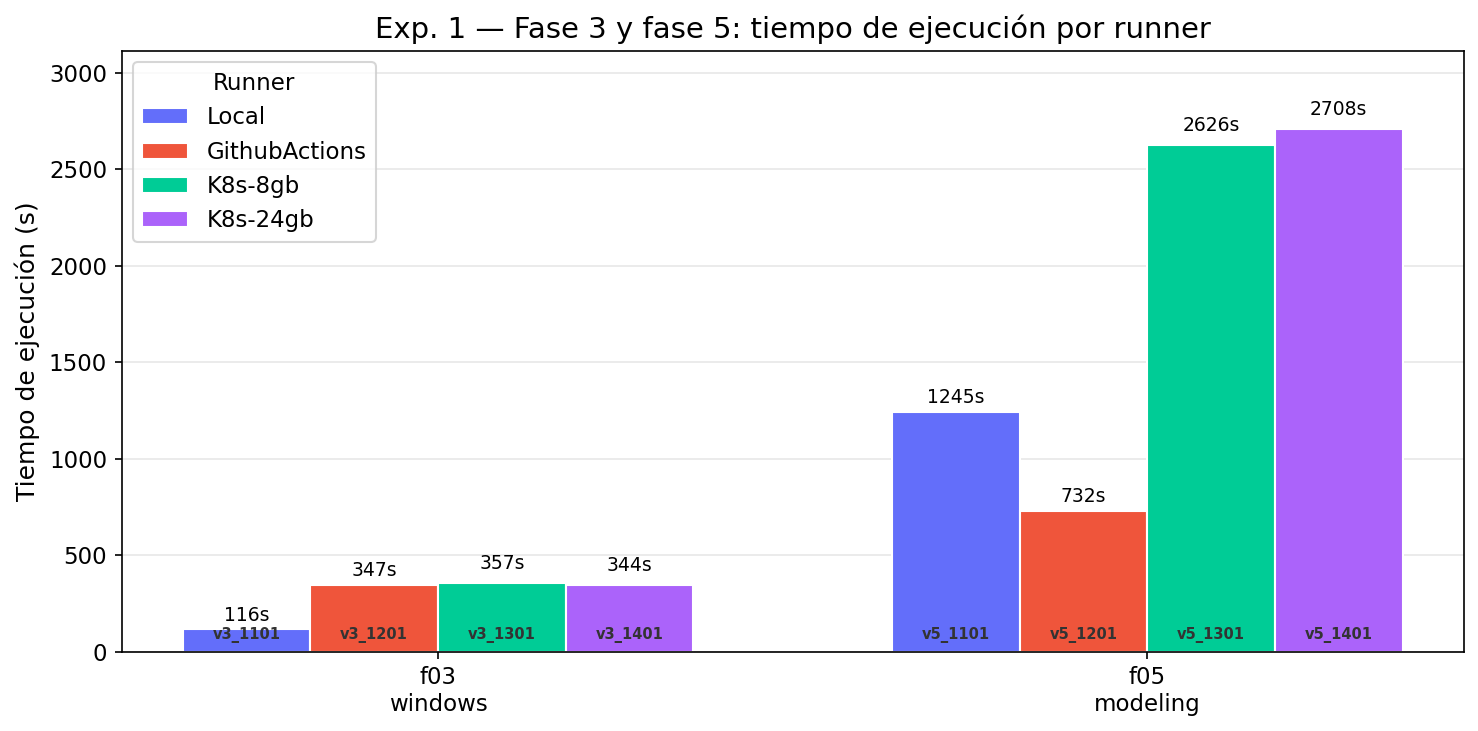
\includegraphics[width=0.95\textwidth]{figures/validacion/comparativa_tiempos_runner.png}
    \caption{Comparativa del tiempo de ejecución de F03 y F05 entre los entornos evaluados.}
    \label{fig:comparativa-tiempos-runner}
\end{figure}

\begin{table}[htbp]
    \centering
    \caption{Plantilla de resumen del Experimento 1 por entorno de ejecución.}
    \label{tab:comparativa-entornos}
    \begin{tabular}{lllll}
        \hline
        \textbf{Entorno} & \textbf{Fase} & \textbf{Variante} & \textbf{Tiempo de ejecución} & \textbf{Estado} \\
        \hline
        Local & [F03/F05] & [variante] & [s] & [estado] \\
        GitHub Actions & [F03/F05] & [variante] & [s] & [estado] \\
        K8s-8gb & [F03/F05] & [variante] & [s] & [estado] \\
        K8s-24gb & [F03/F05] & [variante] & [s] & [estado] \\
        \hline
    \end{tabular}
\end{table}

Esta comparación permite identificar qué entornos son más adecuados para cada tipo de fase. Las fases ligeras pueden beneficiarse de runners pequeños y paralelizables, mientras que las fases con mayor consumo de memoria o CPU pueden requerir perfiles superiores.

\subsection{Experimento 2: saturación y colas}
\label{subsec:validacion-saturacion-colas}

Este experimento comprueba cómo responde el sistema cuando una ráfaga supera la capacidad configurada. Se lanzan ocho variantes equivalentes de F03 sobre el perfil \texttt{K8s-8gb}, limitado a cinco runners simultáneos. En consecuencia, las primeras ejecuciones pueden comenzar en paralelo y las restantes deben permanecer en cola hasta que se libere capacidad. La configuración detallada se muestra en el Anexo~\ref{anexo:exp2-saturacion}.

El análisis separa el tiempo de cola del tiempo efectivo de ejecución. Esta distinción permite verificar que el exceso de demanda se absorbe sin perder variantes ni alterar sus dependencias, y cuantificar la penalización temporal causada por el límite de paralelismo.

\begin{figure}[htbp]
    \centering
    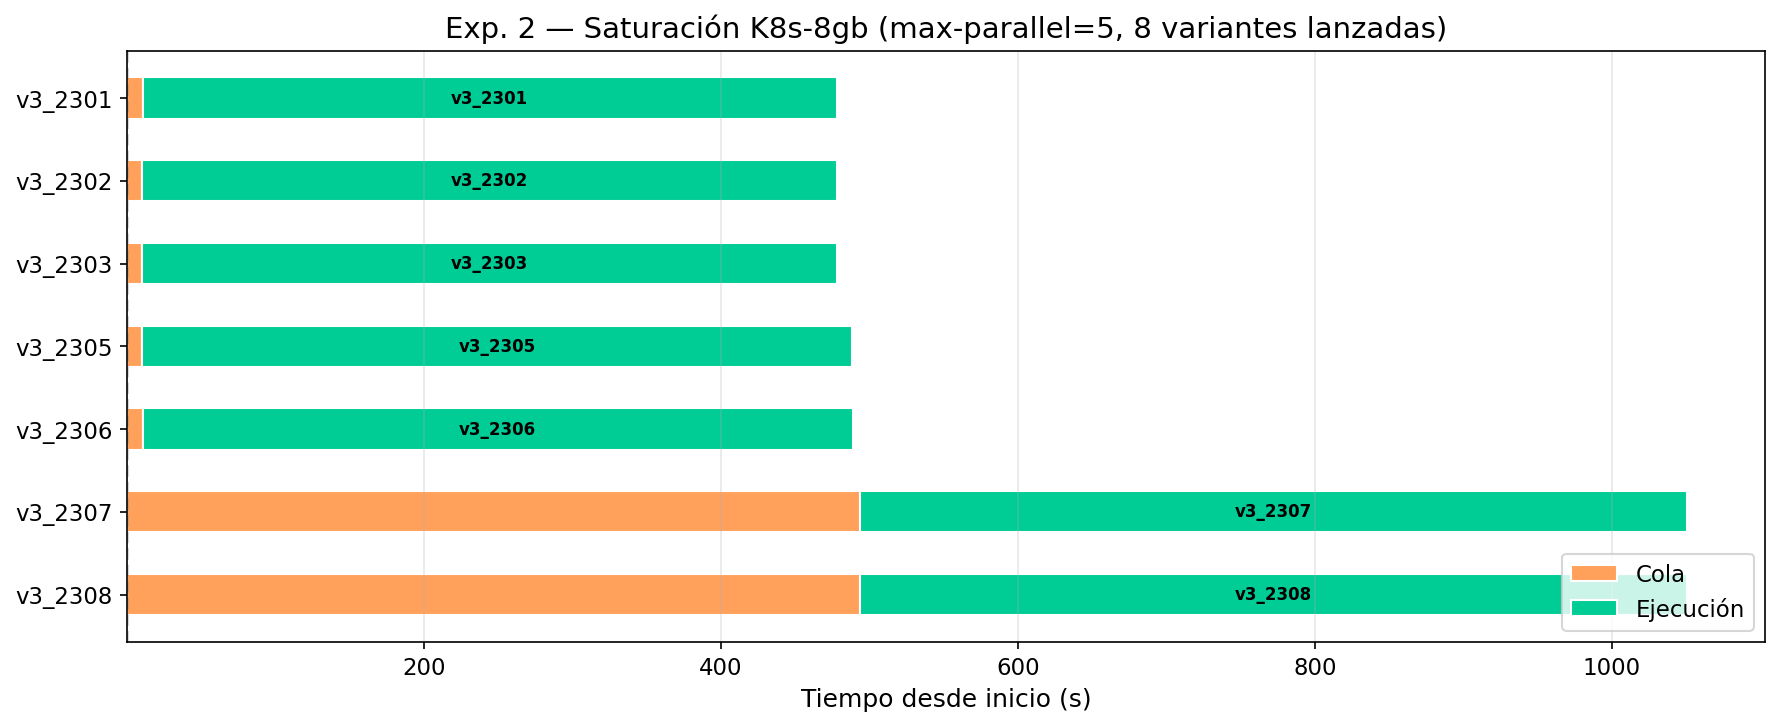
\includegraphics[width=0.95\textwidth]{figures/validacion/robustez_logs_error.png}
    \caption{Cronología de las variantes del Experimento 2, con separación entre espera en cola y ejecución activa.}
    \label{fig:validacion-saturacion-colas}
\end{figure}

\subsection{Experimento 3: ejecución virtual frente a hardware real}
\label{subsec:validacion-virtual-real}

El tercer experimento compara F07 y F08 sobre entornos con ESP32 físico y sobre entornos virtualizados, manteniendo el modelo y el conjunto de datos de entrada. Las variantes y sus relaciones de dependencia se detallan en el Anexo~\ref{anexo:exp3-virtual-real}. Esta prueba incorpora la validación \textit{Hardware-in-the-Loop}: para que una medición sea válida, el runner físico debe recibir el trabajo, acceder al dispositivo y devolver correctamente el resultado al pipeline.

En F07 conviene interpretar por separado el coste de compilación y el de inferencia, puesto que el intervalo de inferencia está condicionado por \texttt{MTI\_MS}. Además del tiempo de ejecución, se contrasta el estado final y la coherencia de los resultados. La comparación determina si el entorno virtual es adecuado para prevalidaciones y qué comprobaciones deben reservarse al dispositivo real.

\begin{figure}[htbp]
    \centering
    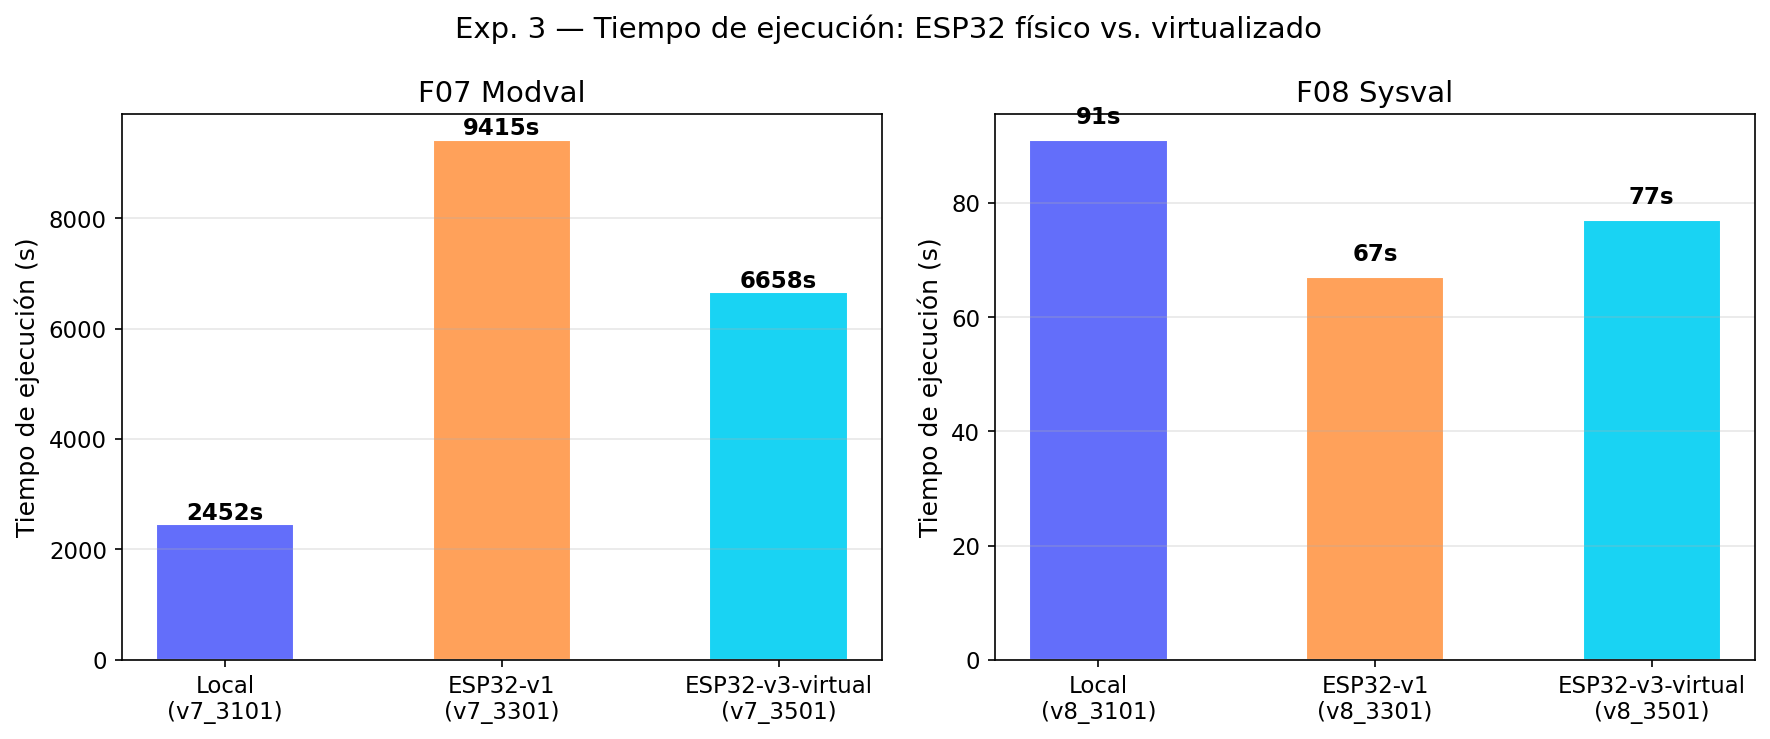
\includegraphics[width=0.95\textwidth]{figures/validacion/arquitectura_hitl_esp32.png}
    \caption{Comparación del tiempo de ejecución de F07 y F08 en entornos ESP32 físicos y virtualizados.}
    \label{fig:validacion-virtual-real}
\end{figure}

\subsection{Experimento 4: valor de la paralelización}
\label{subsec:validacion-paralelizacion}

El último experimento ejecuta el mismo árbol de variantes F01--F04 en dos modalidades: secuencial, con una única ejecución activa, y paralela, respetando las dependencias padre-hija. El árbol y los parámetros de ambas modalidades se recogen en el Anexo~\ref{anexo:exp4-gantt}.

La métrica principal es el \textit{lead time} del lote, medido desde la creación de la primera variante hasta la finalización de la última. A partir de este valor se calcula la aceleración respecto a la ejecución secuencial y se compara el resultado con el límite teórico definido por el camino crítico. El diagrama de Gantt permite comprobar, además, que solo se solapan variantes independientes.

\begin{figure}[htbp]
    \centering
    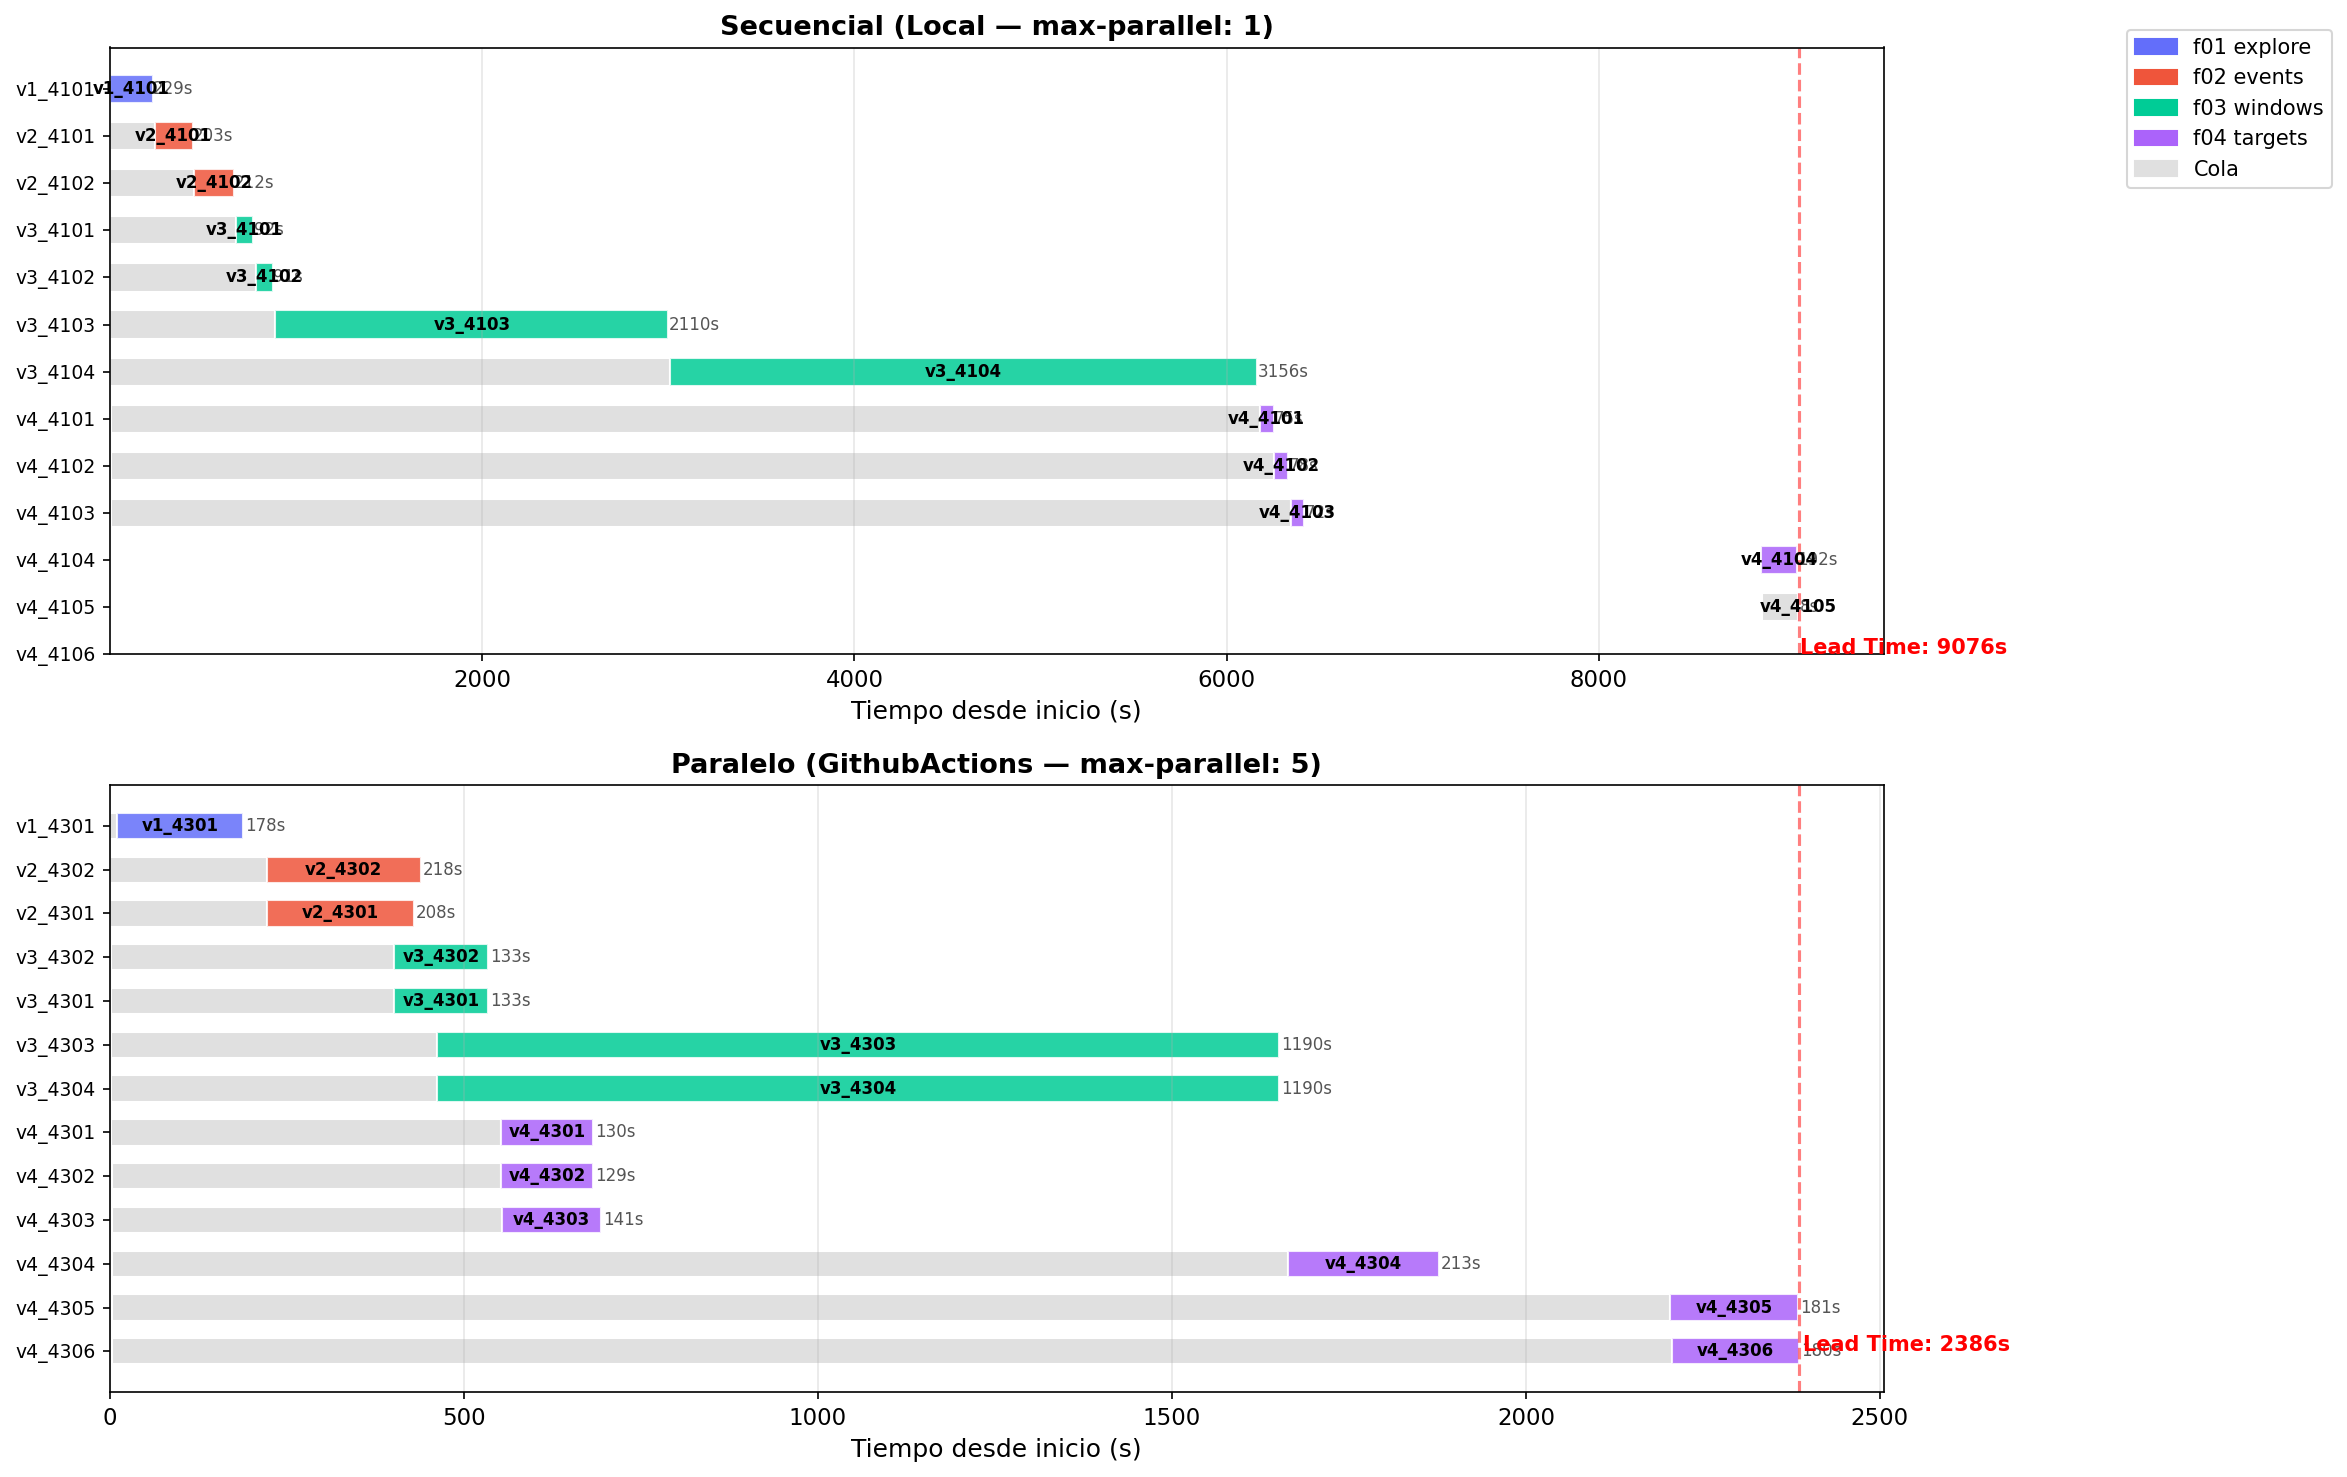
\includegraphics[width=0.95\textwidth]{figures/validacion/paralelizacion_variantes.png}
    \caption{Ejecución secuencial y paralela del árbol de variantes del Experimento 4.}
    \label{fig:validacion-paralelizacion}
\end{figure}

\subsection{Síntesis de resultados}
\label{subsec:sintesis-resultados-validacion}

La Tabla~\ref{tab:sintesis-validacion} reúne los cuatro experimentos y la evidencia utilizada en cada uno. Los valores cuantitativos se completarán con las ejecuciones definitivas seleccionadas en el cuaderno de análisis.

\begin{table}[htbp]
    \centering
    \caption{Síntesis de resultados de la validación experimental.}
    \label{tab:sintesis-validacion}
    \begin{tabular}{p{0.13\textwidth}p{0.25\textwidth}p{0.30\textwidth}p{0.20\textwidth}}
        \hline
        \textbf{Bloque validado} & \textbf{Evidencia} & \textbf{Resultado esperado} & \textbf{Resultado final} \\
        \hline
        Experimento 1 & Tiempos de F03 y F05 por runner & Asignación de recursos caracterizada & [completar] \\
        Experimento 2 & Cronología de cola y ejecución & Saturación gestionada sin pérdida de variantes & [completar] \\
        Experimento 3 & Tiempos y estados de F07--F08 & Diferencias entre ejecución virtual y real cuantificadas & [completar] \\
        Experimento 4 & Diagramas de Gantt y camino crítico & Reducción del \textit{lead time} cuantificada & [completar] \\
        \hline
    \end{tabular}
\end{table}

En conjunto, los experimentos cubren el uso de recursos, la respuesta ante saturación, la ejecución sobre hardware real y el beneficio de la concurrencia. La correcta finalización y el mantenimiento de las dependencias entre variantes proporcionan, dentro de estas mismas pruebas, la evidencia funcional y de trazabilidad necesaria.
